\section{Attitude Controller}\label{sec:AttitudeControllerDesign}
%The attitude controller constitutes an inner loop which receives references for the roll and pitch, from the outer loop which is the $x_{\mathrm{I}}$ and $y_{\mathrm{I}}$ translational controller. As it is decided only to move the drone in one inertial axis at a time, the plus configuration explained in \autoref{chap:Model} \fxnote{Ensure that it matches what is written in the model section}, the yaw reference is always set to zero.\\ 
The attitude response of the quadcopter constitutes a coupled behavior, as all the three Euler angles, $\phi$, $\theta$ and $\psi$, are affected by the same four motor velocities, see \autoref{fig:ControlHeadDiagram}. A state space approach is therefore utilized, as this method is convenient when the system has multiple input and multiple sensed outputs \cite{MultipleInputandoutput}.

The system behavior is represented by means of the linearized model equations. These linearized equations can be represented in state space form, shown in \autoref{xDotLinear} and \ref{yLinear}.
%
\begin{flalign}
	\vec{\dot{x}}&=\vec{A} \  \vec{x} + \vec{B} \  \vec{u}
	\label{xDotLinear} 
\end{flalign}
\begin{flalign}
	\vec{y}&=\vec{C} \  \vec{x} + \vec{D} \  \vec{u}
	\label{yLinear} 
\end{flalign}
%
\begin{where}	
	\va{\vec{x}}{are the states of the system}{}
	\va{\vec{u}}{are the inputs of the system}{}
	\va{\vec{y}}{are the outputs of the system}{}
    \va{\vec{A}}{is the system matrix}{}
    \va{\vec{B}}{is the input matrix}{}
    \va{\vec{C}}{is the output matrix}{}
    \va{\vec{D}}{is the direct transmission term}{}
\end{where}

A block diagram of the state space description can be seen in \autoref{SSBlocks}.
%
\begin{figure}[H]
	\begin{tikzpicture}[ auto,
                       thick,                         %<--setting line style
                       node distance=1.5cm,             %<--setting default node distance
                       scale=1,                     %<--|these two scale the whole thing
                       every node/.style={scale=1}, %<  |(always change both)
                       >=triangle 45 ]                %<--sets the arrowtype
    
    \draw%-----------------------------------------------------------------------------------------
    	%Drawing Input/Output:
    	node[shape=coordinate][](input1) at (0,0){}
    	node[shape=coordinate][](output1) at (9.5,0){}
     	%Drawing the Equation Blocks:   	
      	node(A) at (4.5,-1.5) [block] {A} 
     	node(B) at (1.5,0) [block] {B}
     	node(C) at (6.5,0) [block] {C}
      	node(D) at (4.5,1.5) [block] {D}  
	    node(int) at (4.5,0) [block] {\si{\int}}  
    	%Drawing the Sumation Blocks:	    	 	
    	node(sum1) [sum, right of = B] {\si{\sum}}
    	node(sum2) [sum, right of = C] {\si{\sum}}
    	%Drawing the Feedback/Feedforward Nodes:    	
    	node[shape=coordinate][](FeedforwardNode) at (0.75,0){}
    	node[shape=coordinate][](FeedbackNode) at (5.5,0){}  	
    	     
    ;%---------------------------------------------------------------------------------------------
   
    %Joining the Blocks
  	\draw[->](input1) -- node {u}(B);
  	\draw[->](B) -- node {}(sum1);
  	\draw[->](sum1) -- node {\si{\dot x}}(int);  	
  	\draw[->](int) -- node {x}(C);
  	\draw[->](C) -- node {}(sum2);  	
  	\draw[->](sum2) -- node {y}(output1);
  	
  	\draw[->](FeedforwardNode) |- node{} (D);
  	\draw[->](D) -| node{} (sum2);

  	\draw[-] (FeedbackNode) |- (A);
  	\draw[->] (A)   -| (sum1);

    %Drawing node(s) with \textbullet
    \draw%--------------------------------------------------------------
      node at (input1)  [shift={(-0.08, -0.02 )}] {\large \textbullet}
    	% node at (output1) [shift={( 0.008, -0.02 )}] {\textbullet}
    ;%------------------------------------------------------------------
  \end{tikzpicture}
	\centering
	\caption{Block diagram of the state space representation of the system.}
	\label{SSBlocks}
\end{figure}\vspace{-18pt}
%
The state vector, $\vec{x}$, contains six elements, as there are three attitude second order differential equations, see the linearized \autoref{eq:AngleLincombined1}, \ref{eq:AngleLincombined2} and \ref{eq:AngleLincombined3}. As for mechanical systems, the states are the angular velocities and positions of the system \cite{Stateschosen}.%, as Newton's Second Law is utilized .

The variables in the linearized equations are represented without the symbol $\Delta$, even though they refer to changes around the linearization point.

The size of the input vector, $\vec{u}$, corresponds to the number of inputs, which are the four motor velocities. The output, $\vec{y}$, contains the three angles, $\phi$, $\theta$ and $\psi$. The generated vectors can be seen in \autoref{uVector}.

\begin{minipage}{0.32\linewidth}
	\begin{flalign}
		\vec{x} = 
		\begin{bmatrix}
			\phi \\
			\theta \\ 
			\psi \\
			\dot{\phi} \\
			\dot{\theta} \\
			\dot{\psi} \\
		\end{bmatrix}	\nonumber
		\label{xVector}
	\end{flalign}  
\end{minipage}\hfill
%\hspace{0.03\linewidth}
\begin{minipage}{0.32\linewidth}
	\begin{flalign}
		\vec{y} = 
		\begin{bmatrix}
			\phi \\
			\theta \\ 
			\psi \\
		\end{bmatrix}	\nonumber
		\label{yVector}
	\end{flalign}
\end{minipage}\hfill
%\hspace{0.03\linewidth}
\begin{minipage}{0.32\linewidth}
	\begin{flalign}
		\vec{u}= 
		\begin{bmatrix}
			\omega_1 \\
			\omega_2 \\
			\omega_3 \\
			\omega_4 \\
		\end{bmatrix}\textsl{}
		\label{uVector}
	\end{flalign}
\end{minipage}\hfill

The specific matrices for the description of the angular behavior are obtained from the linearized equations of the system. The size of the input matrix, $\vec{B}$, is $n \times m$, where n is the order of the system and m is the number of inputs. The size of the system matrix, $\vec{A}$, is an $n \times n$ and the output matrix, $\vec{C}$, is an $1 \times n$ matrix. The matrices generated from the linear attitude equations are showed embedded in the state space representation in \autoref{xDotSS} and \ref{ySS}.
%
\begin{flalign}   \label{xDotSS}
	\vec{\dot{x}} &=
	\begin{bmatrix}
		\ 0 & 0 & 0 & 1 & 0 & 0     \ \ \ \\ 
		\ 0 & 0 & 0 & 0 & 1 & 0     \ \ \ \\ 
		\ 0 & 0 & 0 & 0 & 0 & 1     \ \ \ \\
		\ 0 & 0 & 0 & 0 & 0 & 0     \ \ \ \\ 
		\ 0 & 0 & 0 & 0 & 0 & 0     \ \ \ \\ 
		\ 0 & 0 & 0 & 0 & 0 & 0     \ \ \ 		
	\end{bmatrix}
	\vec{x} +
	\begin{bmatrix}
		\ 0 & 0 & 0 & 0      \ \ \ \\ 
		\ 0 & 0 & 0 & 0      \ \ \ \\ 
		\ 0 & 0 & 0 & 0      \ \ \ \\
		\ 0 & \si{-\frac{2 \  k_{th} \  L \  \overline{\omega}_2}{J_x}} & 0 & \si{\frac{2 \  k_{th} \  L \  \overline{\omega}_4}{J_x}}      \ \ \ \\ 
		\ \si{\frac{2 \  k_{th} \  L \  \overline{\omega}_1}{J_y}} & 0 & \si{-\frac{2 \  k_{th} \  L \  \overline{\omega}_3}{J_y}} & 0      \ \ \ \\ 
		\ \frac{2 \  k_d \  {\overline{\omega}_1}}{J_z} & - \frac{2 \  k_d \  {\overline{\omega}_2}}{J_z} & \frac{2 \  k_d \  {\overline{\omega}_3}}{J_z} & - \frac{2 \  k_d \  {\overline{\omega}_4}}{J_z}      \ \ \ 		
	\end{bmatrix}
	\vec{u}
\end{flalign}
\begin{flalign} \label{ySS}
	\vec{y} &=	 
	\begin{bmatrix}
		\ 1 & 0 & 0 & 0 & 0 & 0     \ \ \ \\ 
		\ 0 & 1 & 0 & 0 & 0 & 0     \ \ \ \\ 
		\ 0 & 0 & 1 & 0 & 0 & 0     \ \ \ 		
	\end{bmatrix}
	\vec{x}
\end{flalign}

Before designing the controller, it is convenient to check controllability and observability of the system. For doing so, the controllability and observability matrices shown in \autoref{controlabilityandobservability} are used. 

\begin{minipage}{0.45\linewidth}
\begin{flalign}
\vec{{\mathcal C}} = 
\begin{bmatrix}
\vec{B}&\vec{A}\vec{B}&\vec{A^2}\vec{B}&\vec{A^3}\vec{B}&\vec{A^4}\vec{B}&\vec{A^5}\vec{B} \\	
\end{bmatrix}\nonumber 
\end{flalign}
\end{minipage}\hfill
%\hspace{0.03\linewidth}
\begin{minipage}{0.45\linewidth}
\begin{flalign}
\vec{{\mathcal O}} = 
\begin{bmatrix}
\vec{C} \\
\vec{C}\vec{A} \\
\vec{C}\vec{A}^2 \\
\vec{C}\vec{A}^3 \\
\vec{C}\vec{A}^4 \\
\vec{C}\vec{A}^5 \\		
\end{bmatrix}					\label{controlabilityandobservability} 									
\end{flalign}
\end{minipage}\hfill

The rank of these matrices is six, that is, the number of states. This makes the system both controllable and observable. The entries of the matrices can be seen in \autoref{app:matricesSS}.

The dynamics of the system can be analyzed by looking at the system matrix $\vec{A}$. The eigenvalues of this matrix represent the location of the system's open loop poles. In this case, the system has six poles located in zero, which means that the system is marginally stable. In order to place those poles at a stable location, a state feedback is used. This is combined with an integral controller to be able to set a desired reference, different from zero, for the roll and pitch and reject input disturbances in the three angles. 

%As the output is formed by the three angles, these are the only measured states in the system.
For doing the state feedback, the angular velocities are also needed even though they are not measured. The way of obtaining them is using a reduced order observer. This is done even though the angular velocities could be estimated with a numerical differentiation procedure. The observer is more convenient in case of using on board sensors and by using it, that possibility is kept open. %Furthermore from an learning perspective it is valuable.

This approach has the possibility of designing the state feedback, integral control and the reduced order observer independently. This holds due to the separation principle \cite{ObserverChristoffer}, which states that the closed loop poles of the system are the combination of the state feedback with integral control poles and the observer poles. This implies that the system has 12 closed loop poles.% which states that an observer with gain $\vec{L}$ and a feedback with gain $\vec{F}$ results in 2n closed loop poles \cite{ObserverChristoffer}, where n is the number of states in the system. As a reduced order observer is utilized for estimating the angular velocities, only nine poles are created. 

A block diagram showing the system overview of the attitude controller is shown in \autoref{attitudecontrollerdiagram}. Here the state feedback, the integral control and the reduced order observer can be seen.
\begin{figure}[H]
	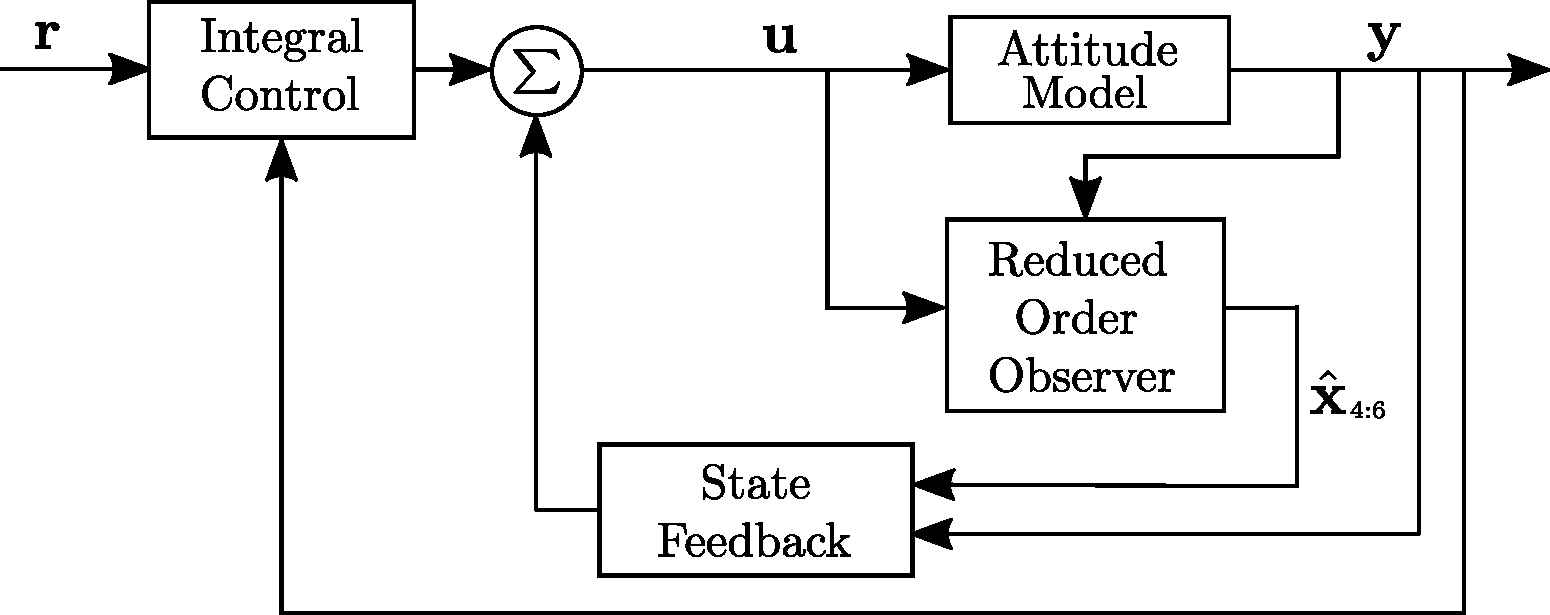
\includegraphics[scale=.45]{figures/AttitudeControlDiagram}
	\centering
	\caption{Control structure for the system, including the state feedback, the integral control and the reduced order observer.}
	\label{attitudecontrollerdiagram}
\end{figure}

In the following subsections, the state feedback with the integral control and then the reduced order observer are designed.

%These show how the output and the states of the system evolve as a function of the current states values and the input applied to the system. \autoref{xDotDiffEq} and \autoref{yDiffEq} show the idea of state space representation.
%
%\begin{flalign}
%	\vec{\dot{x}}(t)&=f(\vec{x}(t),\vec{u}(t))
%	\label{xDotDiffEq} 
%\end{flalign}
%\begin{flalign}
%	\vec{y}(t)&=g(\vec{x}(t),\vec{u}(t)) 
%	\label{yDiffEq} 
%\end{flalign}
%